\clearpage
\section{Multivariate Analysis}
We examine correlations between answers from respondents from borrower and lender countries conditional on respondents socio-demographic characteristics. Macro-economic variables that vary across individual countries are considered in section 5. We estimate the following logit model both for the sample of experts (the WES sample) and the sample of non-experts (the prolific sample). 
\begin{equation*}
    Y_{ij}= \alpha_{j}+ \beta_{j} *D_{i} + \gamma_{j}*X_{i} + \epsilon_{ij}
\end{equation*}
Where $Y_{ij}$ describes the response of individual $i$ to question $j$. Our answer possibilities either allow individuals to state their level of agreement with a statement or whether a statement applies to lender or borrower countries. $Y_{ij}$ takes a value of one if a participant stated either strongly or slightly agree or if a participant stated the lender countries as the responsible party. The dummy variable $D_{i}$ indicates whether the respondents report to have the nationality of one of the borrower countries. We control for individual characteristics $X_{i}$ such as age, level of education, gender and employment status (affiliation for the expert sample). 
We report marginal effects of the dummy variable measuring whether a respondent has the nationality of one of the borrower countries.
%Laura: Was meinst du mit robust standard errors? Wir clustern ja nur als Robustness check
%Schätzen wir nicht mit logit..., rob ?
\\ \\
\textbf{Baseline Results} 
Our baseline results corroborate the findings of our descriptive analysis. \\ 
 \begin{figure}[H]
\begin{center}
     \caption{Intentions of the lender countries}
    
     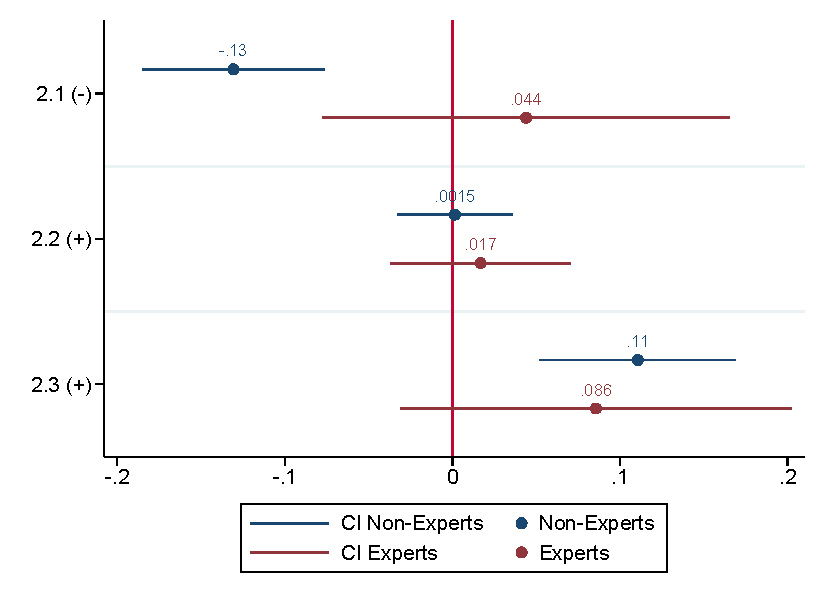
\includegraphics[scale=0.8]{Question2_base.pdf}
     \label{fig:figure6}
      \end{center}
      \tiny
     \tablenotes{The exact wording of the questions were the following.  Question 2.1: The lender countries wanted to help the borrowing countries Question 2.2: The lender countries wanted to help themselves avoid a crisis at home Question 2.3: The lender countries wanted to impose institutional change upon the borrower countries  }
\end{figure}
We examine who initiated and who benefited from the credit relationship. 
Non-experts from borrower countries are 13.2 percentage points less likely to report that the lender countries wanted to help the borrower countries than non-experts from lender countries (\autoref{fig:figure6}). Non-experts from borrower countries are 13 (28) percentage points more likely to report that the lender countries were the driving force behind signing the memorandum (the main beneficiaries of the program) than non-exerts from lender countries (\autoref{fig:figure7}). These marginal effects are statistically significant at the one percent level. We do not find statistically significant effects in the expert sample. \\
\begin{figure}[h!] 
\begin{center}
     \caption{Who initiated and benefited from the rescue program}
     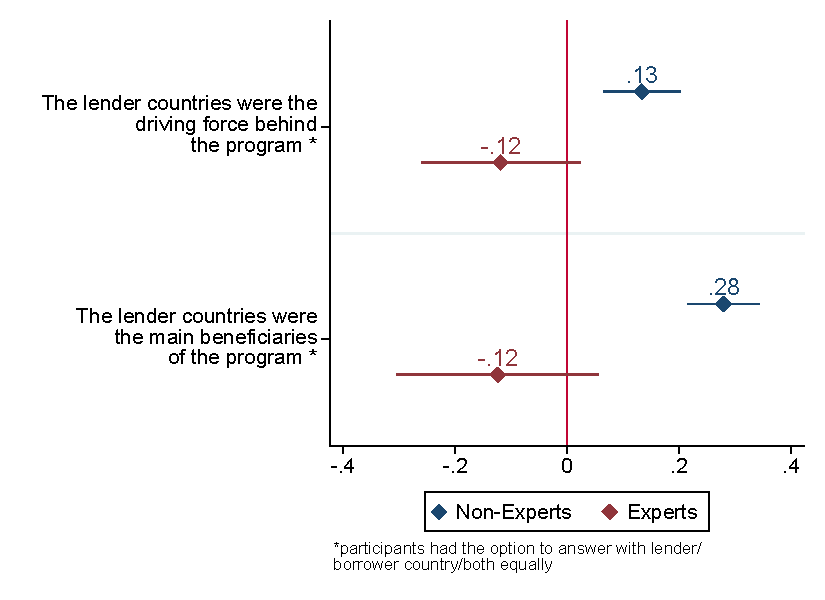
\includegraphics[scale=0.8]{Question3_4_base.pdf}
     \label{fig:figure7}
     \end{center}
     \tiny
     \tablenotes{The sign in parentheses denotes the predicted differential effect.Question 3: Who was the driving force behind signing the memorandum; Question 4: Who was the main beneficiary of the program; Question 7: Who primarily benefited from the loans to Greece}
\end{figure}
We examine how the rescue program influenced the emotions of citizens. Participants from program countries in the non-expert sample are 9.2 and 9.3 percentage points more likely to agree that the rescue experience made them feel guilty and inferior. Further, the probability to agree to "The rescue experience made many citizens in the borrower countries feel exploited" increases by 17 percentage points among citizens from program countries. These marginal effects are statistically significant at the 1 percent level (\autoref{fig:figure8}).  \\
Experts and non-experts from borrower countries do not have a blind spot about the emotions evoked by lender countries (\autoref{fig:figure9}).  \\


 \begin{figure} [h!]
    \begin{center}
    \caption{Sentiments of the borrower countries}
    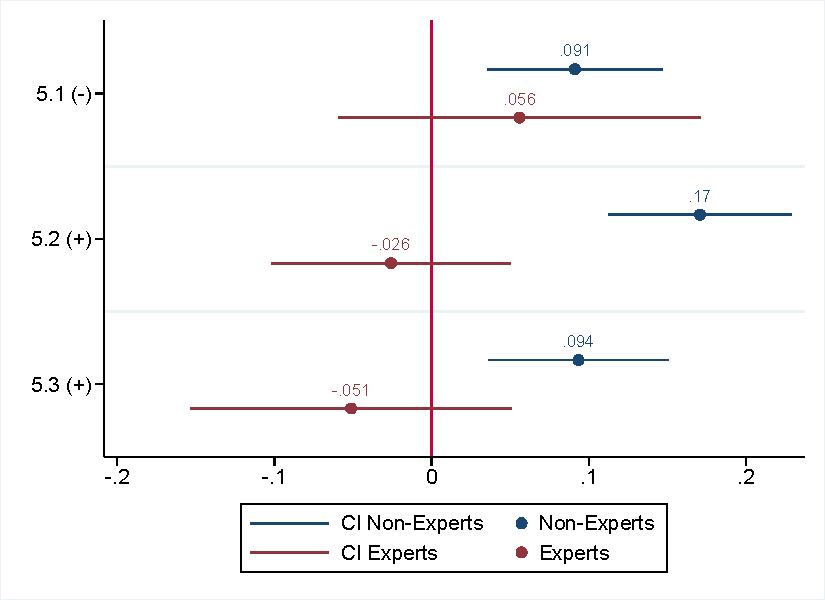
\includegraphics[scale=0.8]{Question5_1_base.pdf}
    \label{fig:figure8}
    \end{center}
    \tiny
    \tablenotes{The exact wording of the questions are the following. Question 5.1: The rescue experience made many citizens in the borrower countries feel guilty; Question 5.2: The rescue experience made many citizens in the borrower countries feel exploited; Question 5.3: The rescue experience made many citizens in the borrower countries feel inferior. }
\end{figure}
\begin{figure}[h!]
\begin{center}
\caption{Sentiments among lender country citizens}

    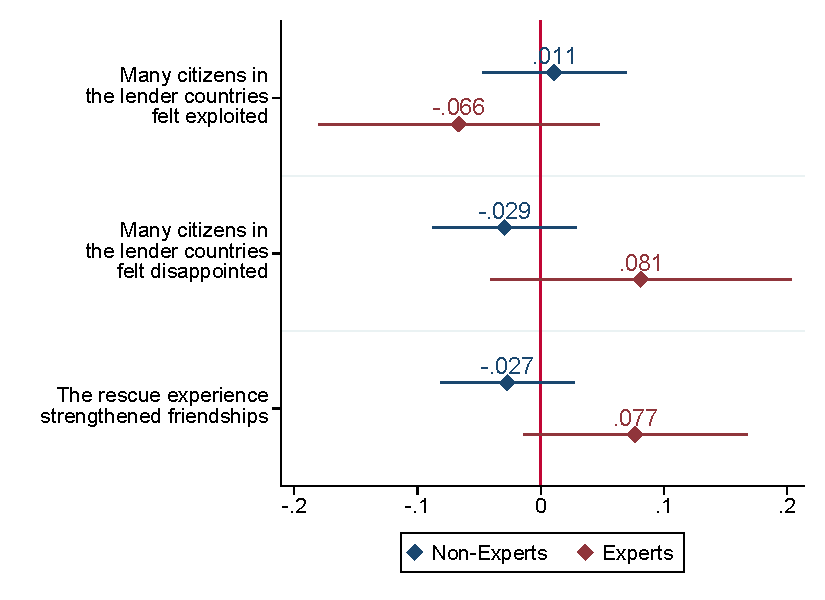
\includegraphics[scale=0.8]{Question5_2_base.pdf}
    \label{fig:figure9}
    \end{center}
    \tiny
    \tablenotes{The sign in parantheses denoted the predicted differential effect. Question 5.4: The rescue experience made many citizens in the lender countries feel exploited; Question 5.5 The rescue experience made many citizens in the lender countries feel disappointed Question 5.6: The rescue experience strengthened friendships between citizens Question 7: Greece will fully pay back it's debt}
\end{figure}
 
%  \begin{figure}
%\caption{Assessment of the emotions the program evoked among different parties}
%\centering
%\begin{minipage}{.5\textwidth}
% 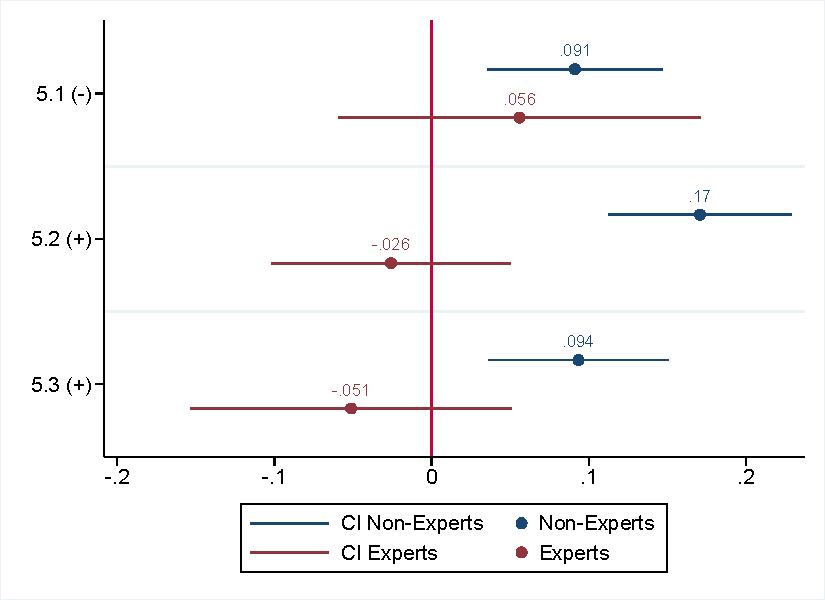
\includegraphics[scale=0.5]{Question5_1_base.pdf}
 %\end{minipage}%
 %\hfill
%\begin{minipage}{.5\textwidth}
%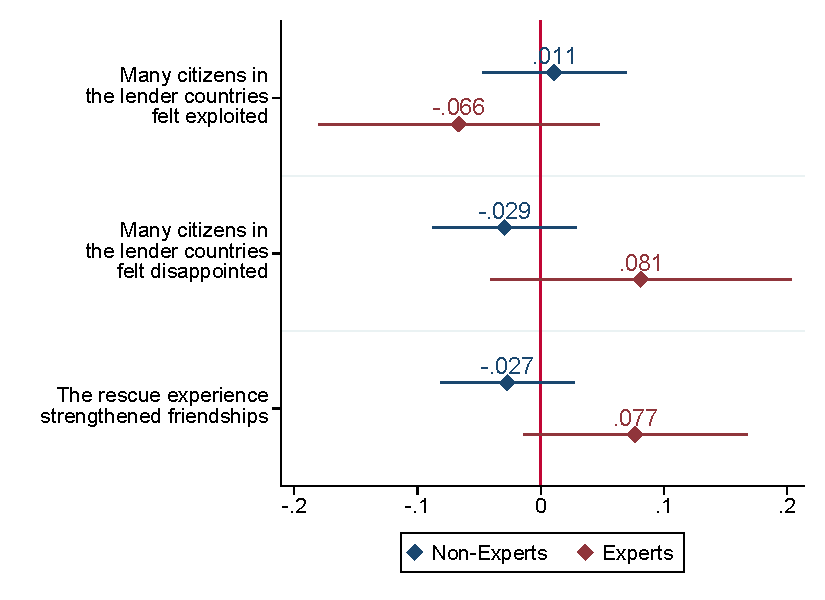
\includegraphics[scale=0.5]{Question5_2_base.pdf}
%\end{minipage}
%\end{figure}

\clearpage
\section{Heterogeneity Analysis}

We investigate explanations for why we only observe a nation-serving bias among our sample of non-experts. 
We examine which socioeconomic characteristics inherent to experts might explain why we do not observe a nation-serving bias among experts. We use subsamples to examine whether individual groups of the participants have a stronger nation-serving bias than others.
\\
 Events experienced at a younger age might have a more defining impact than events experienced at an older age (\cite{baumeister}). Since the European debt crisis was accompanied for example by a high level of youth unemployment it is plausible that the divergences in memory might be more pronounced among the younger generation. Thus, we estimate the effect of belonging to a program country among participants older than 35 among the sample of non-experts.  The effect of the program variable on the likelihood to agree that the lender countries wanted to impose institutional change or that the rescue experience made citizens in the borrower countries feel guilty is smaller and the significance level decreases to 5 percent. For the remaining questions inferences regarding the program effect do not change. 
\\
Participants with a high level of education might have different political attitudes or use different types of media than participants with a low level of education. Hence, we split the non-expert sample and estimate our model only for participants reporting to have completed tertiary education. Inferences regarding the program effect do not change. 
\\
The degree of mobility and exposure to an international environment may well differ between experts and non-experts. Experts working in think tanks or research institutes might live or have studied abroad for some time. Experts might therefore identify less with their nation than non-experts and consequently will not have a strong nation-serving bias. Previous studies such as the one by \cite{bechtel} have shown that having a cosmopolitan attitude was a strong predictor of citizens' attitudes towards the rescue program. Citizens with a cosmopolitan attitude were more willing to accept international redistribution in the form of financial loans than citizens with a less cosmopolitan attitude. We did not include a measure of sharing cosmopolitan attitudes in our survey. However, we know if participants reported to be living in a different country than their country of birth. Overall 541 non-experts reported living in a different country than their country of birth. 437 of these non-experts are from borrower countries and 104 are from lender countries. The fraction of participants living in a different country than their country of birth is quite equally distributed among borrower countries. For lender countries the highest fraction of mobile participants come from Eastern European countries. Estimating our model for this subsample changes the inferences. Divergence between citizens from borrower and lender countries remains in the assessment if lender countries wanted to help borrowing countries and if the rescue experience made the citizens in the borrower countries feel exploited. For the other questions the difference in answers between program- and non-program countries becomes smaller or vanishes. Hence, consistent with previous studies (NIKLAS: WELCHE STUDIEN? NUR BECHTEL ET AL?), participants who are more mobile and more cosmopolitan have a lower nation-serving bias.  \\

We also investigate whether participants' beliefs about the status of their country influence results. One might expect that citizens who are well informed about their country's status as a lender or borrower country might display a stronger nation-serving bias. Restricting the sample to participants who correctly stated whether their country had borrower or lender status does not change the inferences. We also redefine the dummy variable according to citizen's beliefs about the status of their country. We investigate whether we find significant divergence between citizens who believe to live in a lender country and citizens who believe to live in a borrower country. Doing so gives rise to smaller marginal effects of the program dummy variable than in our original baseline estimates. The only significant divergence between participants who believed to be living in lender countries and participants who believed to be living in borrower countries can be found in the assessment of the emotions the rescue program evoked among the lender countries. Identifying as borrower or lender does not drive the results but rather that the recollection of the European debt crisis is influenced by subconscious factors. 
\\
The absence of a nation-serving bias among the expert sample does not seem to be driven by differences in socioeconomic characteristics such as age or education.  However, we find that non-experts who were born in a different country than their current country of residence have a lower degree of nation-serving bias than the full sample. The lack of  a nation-serving bias among the expert sample may be explained by a lower degree of identification with one's nation and hence not feel as part of the group of borrower or lender countries but of the group of experts. 

